\section{Planificación en Multiprocesadores}

En las siguientes secciones se estudia la planificación en sistemas con múltiples procesadores y múltiples núcleos. Primero se analizan los problemas de planificación en multiprocesadores, considerando tanto procesos como hilos. Posteriormente se introduce la planificación en sistemas de tiempo real (RTOS), incluyendo las características de los procesos de tiempo real y algoritmos como \textit{Deadline Scheduling} y \textit{Rate Monotonic Scheduling}.

\subsection{En Multiprocesadores y Multinúcleo}

La presencia de múltiples procesadores introduce nuevos desafíos para el planificador del sistema operativo. Dependiendo de la organización del hardware, los multiprocesadores pueden clasificarse en:
\begin{itemize}
  \item \textit{Multiprocesadores débilmente acoplados (clusters):} cada procesador posee su propia memoria principal y dispositivos de E/S, comunicándose mediante una red.
  \item \textit{Procesadores especializados:} uno o varios procesadores realizan funciones específicas (por ejemplo, E/S) bajo el control de un procesador principal.
  \item \textit{Multiprocesadores fuertemente acoplados:} varios procesadores comparten la memoria principal y son administrados por un único sistema operativo.
\end{itemize}

En esta sección se estudia la planificación en multiprocesadores fuertemente acoplados.

\subsubsection{Granularidad}

La \textit{granularidad} caracteriza el grado de sincronización o comunicación entre procesos o hilos paralelos. Cuanto mayor es la frecuencia de sincronización, más fina es la granularidad y más complejo resulta el trabajo del planificador.

\paragraph{Paralelismo independiente}

No existe sincronización entre procesos, ya que cada uno ejecuta una aplicación distinta. Es el caso típico de un sistema de tiempo compartido, donde varios usuarios ejecutan programas independientes. La disponibilidad de múltiples procesadores reduce el tiempo de respuesta, aunque la planificación es similar a la de un sistema uniprocesador multiprogramado.

\paragraph{Paralelismo de granularidad gruesa y muy gruesa}

Los procesos cooperan ocasionalmente, por lo que la sincronización es poco frecuente. Este tipo de paralelismo puede implementarse mediante procesos concurrentes con pocas modificaciones respecto a un sistema uniprocesador. En general, cuando la comunicación entre procesos es escasa, un sistema distribuido puede ser suficiente; sin embargo, si la interacción aumenta, un multiprocesador resulta más eficiente al evitar la sobrecarga de comunicación por red.

\paragraph{Paralelismo de granularidad media}

Una aplicación se divide en múltiples hilos dentro de un mismo proceso. Los hilos comparten información y deben sincronizarse con frecuencia, por lo que las decisiones de planificación sobre un hilo afectan al rendimiento de toda la aplicación. En consecuencia, la planificación de hilos requiere mecanismos más sofisticados que la planificación tradicional de procesos.

\paragraph{Paralelismo de granularidad fina}

Representa el mayor nivel de paralelismo y sincronización. Las tareas interactúan continuamente, por lo que la planificación es considerablemente más compleja y suele requerir técnicas especializadas de programación paralela.

\subsection{Aspectos de Diseño}

La planificación en un multiprocesador involucra tres problemas relacionados:
\begin{enumerate}
  \item Asignación de procesos a los procesadores.
  \item Multiprogramación en cada procesador.
  \item Despacho del proceso seleccionado.
\end{enumerate}

La estrategia utilizada depende principalmente de la granularidad del paralelismo y de la cantidad de procesadores disponibles.

\subsubsection{Asignación de procesos a los procesadores}

En multiprocesadores homogéneos (todos los procesadores poseen el mismo acceso a memoria y dispositivos de E/S), los procesadores pueden considerarse un recurso compartido al que los procesos se asignan según sea necesario.

Existen dos estrategias principales:
\begin{itemize}
  \item \textbf{Asignación estática:} cada proceso permanece asociado al mismo procesador durante toda su ejecución. Cada procesador mantiene su propia cola de listos, reduciendo la sobrecarga de planificación y permitiendo técnicas como la \textit{planificación por grupos} (\textit{gang scheduling}). Sin embargo, puede producir desbalance de carga, dejando procesadores ociosos mientras otros acumulan procesos.
  \item \textbf{Asignación dinámica:} los procesos se extraen de una cola global o pueden migrarse entre las colas de distintos procesadores (\textit{balanceo dinámico de carga}). De esta manera se mejora la utilización de los procesadores y se evita el desbalance. Sistemas como Linux utilizan este enfoque.
\end{itemize}

\subsubsection{Organización del planificador}

Existen dos arquitecturas principales para coordinar la planificación:
\begin{itemize}
  \item \textbf{Maestro--esclavo:} un único procesador ejecuta el núcleo del sistema operativo y realiza todas las decisiones de planificación. Los demás procesadores ejecutan procesos de usuario y solicitan servicios al procesador maestro cuando es necesario. Su implementación es sencilla, pero presenta dos inconvenientes: el maestro constituye un punto único de falla y puede convertirse en un cuello de botella.
  \item \textbf{Entre pares:} cualquier procesador puede ejecutar código del núcleo y realizar planificación. Esto mejora la escalabilidad y elimina el cuello de botella del procesador maestro, aunque incrementa la complejidad del sistema operativo, que debe sincronizar el acceso a las colas de procesos y evitar condiciones de carrera durante la asignación de recursos.
\end{itemize}

En la práctica existen soluciones intermedias, como dedicar varios procesadores a tareas del núcleo o diferenciar el tratamiento de procesos del sistema y de usuario mediante prioridades y políticas de planificación.

\subsubsection{Uso de la multiprogramación en cada procesador}

Cuando un proceso permanece asignado al mismo procesador durante toda su ejecución, surge la pregunta de si dicho procesador debe ejecutar varios procesos mediante multiprogramación.

En aplicaciones con paralelismo independiente o de granularidad gruesa, la respuesta es afirmativa: la multiprogramación permite mantener una alta utilización del procesador cuando un proceso se bloquea por operaciones de E/S o sincronización.

Sin embargo, en aplicaciones de granularidad media (basadas en múltiples hilos) y en sistemas con muchos procesadores, maximizar la utilización de cada procesador deja de ser el objetivo principal. En estos casos resulta más importante maximizar el rendimiento global de las aplicaciones, ya que una aplicación paralela puede degradar su desempeño si sus hilos no pueden ejecutarse simultáneamente.

\subsubsection{Despacho de procesos}

Una vez asignados los procesos a los procesadores, el planificador debe decidir cuál ejecutar. Mientras que en sistemas uniprocesador suelen emplearse algoritmos complejos basados en prioridades o historial de ejecución, en multiprocesadores estos mecanismos ofrecen beneficios mucho menores y aumentan la sobrecarga del sistema.

Por ello, en muchos casos resulta preferible utilizar algoritmos de planificación más simples, especialmente cuando el número de procesadores es elevado.

\subsection{Planificación de procesos}

En los multiprocesadores tradicionales los procesos no suelen quedar asociados permanentemente a un procesador. Normalmente existe una cola global de procesos listos (o varias colas por prioridad) desde la cual cualquier procesador puede seleccionar el siguiente proceso a ejecutar.

Diversos estudios muestran que, a medida que aumenta el número de procesadores, la elección del algoritmo de planificación tiene un impacto cada vez menor sobre el rendimiento del sistema. La presencia de múltiples procesadores reduce el efecto negativo de procesos con ráfagas largas de CPU, ya que otros procesos pueden ejecutarse simultáneamente en procesadores diferentes.

Como consecuencia, algoritmos sencillos como \textit{FCFS} o \textit{FCFS con prioridades estáticas} suelen proporcionar un rendimiento comparable al de algoritmos más complejos, con una menor sobrecarga de planificación.

\begin{figure}[!ht]
  \centering
  \begin{subfigure}[c]{0.45\textwidth}
    \centering
    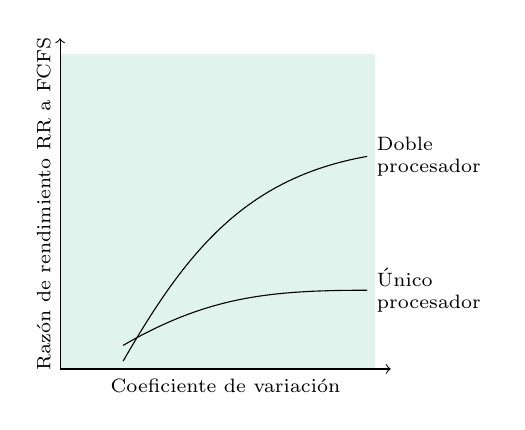
\begin{tikzpicture}[font=\scriptsize]
      \fill[white!95!blue!93!green] (0,0) rectangle (4,4);
      \draw[->] (0,0) -- node[below]{Coeficiente de variación} (4.2,0);
      \draw[->] (0,0) -- node[above,sloped]{Razón de rendimiento RR a FCFS} (0,4.2);
      \draw (0.8,0.3) to[out=30,in=180] (3.9,1) node[right,text width=1.4cm]{Único\\procesador};
      \draw (0.8,0.1) to[out=60,in=190] (3.9,2.7) node[right,text width=1.4cm]{Doble\\procesador};
    \end{tikzpicture}
    \caption{Comparación de RR y FCFS.}
  \end{subfigure}
  \hspace{5mm}
  \begin{subfigure}[c]{0.45\textwidth}
    \centering
    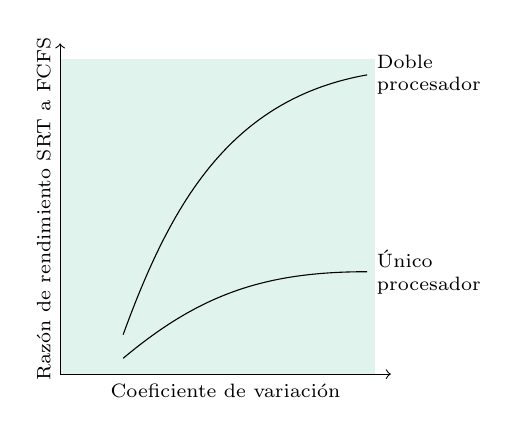
\begin{tikzpicture}[font=\scriptsize]
      \fill[white!95!blue!93!green] (0,0) rectangle (4,4);
      \draw[->] (0,0) -- node[below]{Coeficiente de variación} (4.2,0);
      \draw[->] (0,0) -- node[above,sloped]{Razón de rendimiento SRT a FCFS} (0,4.2);
      \draw (0.8,0.2) to[out=40,in=180] (3.9,1.3) node[right,text width=1.4cm]{Único\\procesador};
      \draw (0.8,0.5) to[out=70,in=190] (3.9,3.8) node[right,text width=1.4cm]{Doble\\procesador};
    \end{tikzpicture}
    \caption{Comparación de SRT y FCFS.}
  \end{subfigure}
  \caption{Comparación del rendimiento de distintos algoritmos de planificación en sistemas con uno y varios procesadores. A medida que aumenta el número de procesadores, las diferencias entre algoritmos como FCFS y Round Robin disminuyen, haciendo que políticas simples sean suficientes en muchos casos.}
\end{figure}

\subsection{Planificación de hilos}

Los hilos permiten separar la ejecución del resto de los recursos de un proceso, posibilitando que varias tareas de una misma aplicación se ejecuten concurrentemente dentro del mismo espacio de direcciones.

En un sistema uniprocesador, los hilos mejoran la estructura de los programas y permiten solapar operaciones de E/S con cómputo, con un costo de cambio de contexto inferior al de los procesos. En un multiprocesador, además, permiten explotar el paralelismo real ejecutando simultáneamente distintos hilos de una misma aplicación. En aplicaciones con alta interacción entre hilos (granularidad media), la política de planificación influye significativamente en el rendimiento.

Las principales estrategias de planificación de hilos son:
\begin{itemize}
  \item \textit{Compartición de carga (\textit{Load Sharing}):} los hilos se almacenan en una cola global y cualquier procesador libre puede ejecutar el siguiente hilo disponible.
  \item \textit{Planificación por grupos (\textit{Gang Scheduling}):} todos los hilos relacionados de una aplicación se ejecutan simultáneamente en distintos procesadores.
  \item \textit{Asignación dedicada de procesadores:} cada aplicación recibe un conjunto fijo de procesadores durante toda su ejecución, normalmente uno por hilo.
  \item \textit{Planificación dinámica:} el número de hilos asignados a una aplicación puede modificarse durante su ejecución según la carga del sistema.
\end{itemize}

\subsubsection{Compartición de carga}

Es la estrategia más simple y una de las más utilizadas en multiprocesadores. Mantiene una cola global de hilos listos, desde la cual cada procesador obtiene trabajo cuando queda libre.

Sus principales ventajas son:
\begin{itemize}
  \item Distribuye automáticamente la carga entre los procesadores.
  \item No requiere un planificador centralizado.
  \item Puede combinarse con cualquier política de planificación, como FCFS o prioridades.
\end{itemize}
Las políticas más comunes para organizar la cola global son:
\begin{itemize}
  \item \textit{FCFS:} los hilos se ejecutan en orden de llegada hasta bloquearse o finalizar.
  \item \textit{Menor número de hilos primero:} se priorizan las aplicaciones que poseen menos hilos pendientes de ejecución.
  \item \textit{Versión apropiativa:} igual que la anterior, pero un nuevo trabajo puede interrumpir la ejecución de otro con menor prioridad.
\end{itemize}

Estudios experimentales muestran que, en la mayoría de los casos, \textit{FCFS} ofrece un mejor rendimiento que las otras variantes de \textit{Load Sharing}. No obstante, la \textit{Gang Scheduling} suele obtener resultados superiores cuando existe una elevada coordinación entre los hilos.

Las principales desventajas de \textit{Load Sharing} son:
\begin{itemize}
  \item La cola global puede convertirse en un cuello de botella cuando muchos procesadores intentan acceder a ella simultáneamente.
  \item Un hilo apropiado puede reanudarse en un procesador distinto, reduciendo la eficiencia de las memorias caché locales.
  \item Los hilos de una misma aplicación pueden ejecutarse en instantes diferentes, perjudicando el rendimiento cuando requieren sincronización frecuente.
\end{itemize}

Una variante consiste en mantener una cola local para cada procesador y una cola global compartida. Cada procesador consulta primero su cola local, reservada para hilos vinculados a dicho procesador, y luego la cola global. Esta organización mejora la localidad de referencia y facilita la implementación de técnicas como la planificación por grupos.

\subsubsection{Planificación por grupos}

La \textit{planificación por grupos} (Gang Scheduling) consiste en ejecutar simultáneamente, en distintos procesadores, todos los hilos relacionados de una misma aplicación. Esta técnica es especialmente útil en aplicaciones con paralelismo de granularidad media o fina, donde los hilos requieren una sincronización frecuente.

Sus principales ventajas son:
\begin{itemize}
  \item Reduce los bloqueos debidos a la sincronización entre hilos, ya que todos pueden ejecutarse al mismo tiempo.
  \item Disminuye la cantidad de cambios de contexto y, por lo tanto, la sobrecarga de planificación.
  \item Facilita el acceso compartido a recursos, reduciendo el costo de sincronización en determinadas operaciones.
\end{itemize}

Si un hilo necesita sincronizarse con otro que aún no está ejecutándose, deberá esperar hasta que el planificador le asigne un procesador, degradando considerablemente el rendimiento. La planificación por grupos evita este problema al garantizar la ejecución simultánea de todos los hilos cooperantes.

La implementación de esta técnica requiere asignar procesadores a cada aplicación. Una estrategia sencilla consiste en repartir el tiempo de CPU entre las aplicaciones mediante \textit{time slicing}. Sin embargo, asignar el mismo tiempo a todas las aplicaciones puede desperdiciar recursos cuando poseen distinta cantidad de hilos.

Una alternativa más eficiente consiste en asignar tiempo de procesador de forma proporcional al número de hilos de cada aplicación. De este modo se reduce el tiempo en que algunos procesadores permanecen inactivos y se mejora la utilización global del sistema.

\begin{figure}[!ht]
  \centering
  \includegraphics[width=0.7\textwidth]{chapters/03_unit/media/gang_scheduling.pdf}
  \caption{Comparación entre una asignación uniforme del tiempo de CPU y una asignación ponderada por la cantidad de hilos. La planificación ponderada reduce el tiempo en que algunos procesadores permanecen ociosos, mejorando la utilización del multiprocesador.}
\end{figure}

\subsection{Asignación dedicada de procesadores}

La \textit{asignación dedicada de procesadores} es una estrategia extrema de la \textit{Gang Scheduling}. Cuando una aplicación comienza a ejecutarse, se le asigna un conjunto fijo de procesadores, uno por hilo, que permanecen dedicados exclusivamente a dicha aplicación hasta su finalización.

A primera vista esta política parece ineficiente, ya que si un hilo se bloquea por una operación de E/S o por sincronización, el procesador asignado permanece inactivo y no puede ejecutar otros procesos. Sin embargo, presenta dos ventajas importantes:
\begin{itemize}
  \item En sistemas con decenas o cientos de procesadores, maximizar la utilización individual de cada procesador deja de ser el objetivo principal; resulta más importante mejorar el rendimiento global de las aplicaciones.
  \item Al eliminar prácticamente todos los cambios de contexto durante la ejecución de una aplicación, se reduce la sobrecarga del sistema y se mejora significativamente su desempeño.
\end{itemize}
Diversos estudios muestran que el rendimiento disminuye cuando el número de hilos activos supera el número de procesadores disponibles. En ese caso aumenta la frecuencia de apropiaciones (\textit{preemption}) y replanificaciones, lo que provoca:
\begin{itemize}
  \item Mayor cantidad de cambios de contexto.
  \item Esperas por hilos suspendidos dentro de secciones críticas.
  \item Pérdida de eficiencia de la memoria caché.
\end{itemize}

Por ello, una estrategia efectiva consiste en limitar el número de hilos activos al número de procesadores del sistema, especialmente en aplicaciones paralelas que pueden distribuir su trabajo mediante colas de tareas.

La asignación dedicada de procesadores y la \textit{Gang Scheduling} abordan el problema desde la perspectiva de la \textit{asignación de procesadores}. Este problema es análogo a la asignación de marcos de página en memoria: el sistema debe decidir cuántos procesadores asignar a cada aplicación para mantener un rendimiento adecuado.

Se define el \textit{conjunto activo de trabajo} (\textit{activity working set}) como el número mínimo de hilos que deben ejecutarse simultáneamente para que una aplicación progrese eficientemente. Si no se asignan suficientes procesadores pueden aparecer dos problemas:
\begin{itemize}
  \item \textit{Thrashing de procesadores:} los hilos necesarios se suspenden mutuamente de forma reiterada, provocando continuas replanificaciones y bajo rendimiento.
  \item \textit{Fragmentación de procesadores:} quedan procesadores libres, pero en una cantidad insuficiente o con una distribución que impide satisfacer las necesidades de las aplicaciones en espera.
\end{itemize}

Las técnicas de \textit{Gang Scheduling} y asignación dedicada buscan minimizar ambos problemas mediante una asignación más eficiente de los procesadores.

\begin{table}[!ht]
  \centering
  \begin{tabular}{c|c|c}
    \makecell{Número de hilos \\ por aplicación} & 
    \makecell{Multiplicación \\ de matriz} & 
    FFT \\ 
    \hline 
    1 & 1 & 1 \\ 
    2 & 1.8 & 1.8 \\
    4 & 3.8 & 3.8 \\
    8 & 6.5 & 6.1 \\
    12 & 5.2 & 5.1 \\
    16 & 3.9 & 3.8 \\
    20 & 3.3 & 3 \\
    24 & 2.8 & 2.4 \\
  \end{tabular}
  \caption{El rendimiento de aplicaciones paralelas aumenta mientras el número de hilos activos no supere la cantidad de procesadores disponibles. Cuando existen más hilos que procesadores, la sobrecarga por apropiaciones y cambios de contexto degrada significativamente el desempeño.}
\end{table}

\subsubsection{Planificación dinámica}

En la \textit{planificación dinámica}, el número de hilos de una aplicación puede modificarse durante su ejecución. Esto permite que el sistema operativo adapte la asignación de procesadores a la carga del sistema, mejorando la utilización de los recursos.

En este enfoque, tanto el sistema operativo como la aplicación participan en la planificación:
\begin{itemize}
  \item El \textit{sistema operativo} decide cuántos procesadores asignar a cada aplicación.
  \item La \textit{aplicación} decide qué tareas ejecutar con los procesadores asignados y qué hilos suspender cuando pierde procesadores.
\end{itemize}
La asignación de procesadores sigue una política sencilla:
\begin{enumerate}
  \item Si existen procesadores libres, se asignan a la aplicación que los solicita.
  \item Si no hay procesadores disponibles, una nueva aplicación recibe al menos un procesador, retirándolo de otra aplicación que posea más de uno.
  \item Las solicitudes no satisfechas permanecen pendientes hasta que algún procesador quede disponible o la aplicación cancele la solicitud.
  \item Cuando se liberan procesadores, primero se atienden las aplicaciones que aún no poseen ninguno y luego el resto de las solicitudes en orden \textit{FCFS}.
\end{enumerate}

Esta estrategia puede ofrecer un mejor rendimiento que la \textit{Gang Scheduling} o la asignación dedicada de procesadores en aplicaciones capaces de adaptar dinámicamente su paralelismo. Sin embargo, la mayor complejidad y la sobrecarga asociada a este mecanismo pueden reducir parte de sus ventajas.

\subsection{Planificación de hilos en sistemas multinúcleo}

Los sistemas operativos modernos, como Windows y Linux, planifican los hilos en sistemas multinúcleo de forma similar a los multiprocesadores, distribuyendo la carga entre los núcleos para mantenerlos ocupados. Sin embargo, esta estrategia no siempre aprovecha al máximo la arquitectura multinúcleo.

A medida que aumenta el número de núcleos, adquiere mayor importancia reducir los accesos a la memoria principal. Para ello se aprovecha la jerarquía de memorias caché, cuya organización influye directamente en las decisiones de planificación.

En muchas arquitecturas multinúcleo, algunos niveles de caché son privados de cada núcleo mientras que otros son compartidos por grupos de núcleos. En consecuencia, la ubicación de los hilos puede afectar significativamente el rendimiento.

\begin{figure}[!ht]
    \centering
    \includegraphics[width=0.8\textwidth]{chapters/03_unit/media/cache_levels.pdf}
    \caption{Ejemplo de jerarquía de caché en un procesador multinúcleo. Cada núcleo posee una caché L1 privada, algunos grupos de núcleos comparten una caché L2 y todos los núcleos comparten una caché L3. La planificación de hilos debe considerar esta organización para mejorar la localidad y reducir la contención de caché.}
\end{figure}

Se distinguen dos situaciones principales:
\begin{itemize}
  \item \textit{Compartición cooperativa de recursos:} varios hilos acceden a los mismos datos. Conviene ejecutarlos en núcleos que compartan caché para aprovechar la localidad de referencia y reducir los accesos a memoria principal.
  \item \textit{Contención de recursos:} varios hilos compiten por el espacio de una misma caché compartida. En este caso es preferible distribuirlos entre núcleos que no compartan caché para evitar reemplazos frecuentes y degradación del rendimiento.
\end{itemize}
Por ello, la planificación en sistemas multinúcleo debe equilibrar dos objetivos: mantener los núcleos ocupados y optimizar el uso de la memoria caché. El desarrollo de algoritmos de planificación sensibles a la jerarquía de caché (\textit{cache-aware scheduling}) y a la contención (\textit{contention-aware scheduling}) constituye un área activa de investigación.

